\chapter{Trave: SLE}\label{chap:traveSLE}

Gli stati limite di esercizio oggetto di verifica in questo documento si limitano a:
\begin{itemize}
	\item stato limite di limitazione delle tensioni;
	\item stato limite di fessurazione;
	\item stato limite di deformazione.
\end{itemize}

Tutti gli stati limite sono regolati dalle \ntc e dalla \circolare con alcuni richiami alle \ec in particolar modo per quanto riguarda la classificazione delle condizioni ambientali.

\section{Stato limite di limitazione delle tensioni}\label{sec:SLE_tensioni}
Lo stato limite di limitazione delle tensioni è descritto al punto \textbf{4.1.2.2.5} delle \ntc e nel punto \textbf{C4.1.2.2.5} della \textbf{CIRC. N. 7}. Le ipotesi alla base sono:
\begin{itemize}
	\item comportamento elastico - lineare dei materiali;
	\item resistenza a trazione del calcestruzzo trascurabile;
	\item ipotesi di Bernoulli - Navier per cui le sezioni ruotano, traslano e rimangono piane;
	\item coefficiente di omogeneizzazione $n = \frac{E_s}{E_c} = 15$ che tiene conto degli effetti della viscosità nel calcestruzzo.
\end{itemize}

La verifica sulle tensioni va eseguita per le combinazioni delle azioni di tipo \textit{caratteristica} (o combinazione rara) e \textit{quasi permanente}. Per la prima le tensioni nel calcestruzzo devono essere inferiori a
\begin{equation}
	\label{eq:sigma_c_riferimento_rara}
	\sigma_c^R = 0.60\,f_{ck} = 0.60\cdot 25\,MPa = 15\,MPa
\end{equation}
mentre per la seconda 
\begin{equation}
	\label{eq:sigma_c_riferimento_rara}
	\sigma_c^R = 0.45\,f_{ck} = 0.45\cdot 25\,MPa = 6.75\,MPa
\end{equation}

Per quanto riguarda la tensione massima nell'acciaio, la normativa italiana fissa il limite per la \textit{combinazione caratteristica} pari a
\begin{equation}
	\label{eq:sigma_s_riferimento_rara}
	\sigma_s^R = 0.8\,f_{yk} = 0.80\cdot 450\,MPa = 360\,MPa
\end{equation}

\begin{figure}
	\centering
	\subfloat[\emph{Andamento del campo deformativo e tensionale}]{
		\begin{tikzpicture}[scale=.1]
			
			\draw[thick=2] (0,0) rectangle (30,50);
			\draw[very thick] (4, 4) --node[above]{$A_s$} ++(22,0);
			\draw[very thick] (4, 46) --node[below]{$A'_s$}++(22,0);
			\draw[|-|] (-4,4) -- node [left] {$d$} (-4,50);
			\draw[|-|] (-6,0) -- node [left] {$d'$} (-6,4);
			\draw[|-|] (-6,50) -- node [left] {$d''$} (-6,46);
			\draw[|-|] (-12,0) -- node [left] {$h$} (-12,50);
			\draw[|-|] (0, -4) -- node[below] {$b$} (30, -4);
			\draw[thin, dashed] (30,0) -- ++(80,0);
			\draw[thin, dashed] (30,50) -- ++(80,0);
			
			\draw[thin, -latex] (15,22.5) -- ++(0, 35) node [right] {$y$};
			
			\draw[thick] (58,50) -- (58,0);
			\draw[thick] (80,50) -- (40,0);
			\draw[thick] (58,50)-- node[above] {$\epsilon_c^{sup}$}(80,50);
			\draw[thick] (40,0)-- node[below] {$\epsilon_c^{inf}$}(58,0);
			
			\draw[thick] (58,46)-- node[below] {$\epsilon'_s$}(77,46);
			\draw[thick] (43,4)-- node[above] {$\epsilon_s$}(58,4);
			\draw[thick, C01] (0,22.5)node[above right]{$n$} --++(120,0) node[above left] {$n$};
			\draw[|-|, thin] (35,50) -- node[right] {$x$} (35,22.5);
			
			\begin{scope}[shift={(40,0)}]
				\draw[thick] (58,50) -- (58,0);
				\draw[thick] (80,50) -- (58,22.5);
				\draw[thick, dashed] (58,22.5) -- (40,0);
				\draw[thick] (58,50)-- node[above] {$\sigma_c$}(80,50);
				
				\draw[thick] (58,46)-- node[below] {$\dfrac{\sigma'_s}{n}$}(77,46);
				\draw[thick] (43,4)-- node[above right] {$\dfrac{\sigma_s}{n}$}(58,4);
			\end{scope}
		\end{tikzpicture}}\\
	\subfloat[\emph{Risultanti delle tensioni}]{
		\begin{tikzpicture}[scale=.14]
			
			\draw[thick=2] (-10,50)--(30,50) -- (30,0) -- (-10,0);
			\draw[thick=2, dash dot] (-10,0) -- (-10,50);
			\draw[very thick] (-10, 4) --node[above]{$A_s$} ++(36,0);
			\draw[very thick] (-10, 46) --node[below]{$A'_s$}++(36,0);
			% 			\draw[|-|] (-4,4) -- node [left] {$d$} (-4,50);
			% 			\draw[|-|] (-6,0) -- node [left] {$d'$} (-6,4);
			% 			\draw[|-|] (-6,50) -- node [left] {$d''$} (-6,46);
			% 			\draw[|-|] (-10,0) -- node [left] {$h$} (-10,50);
			% 			\draw[|-|] (0, -4) -- node[below] {$b$} (30, -4);
			
			\draw[|-|] (-14,4) -- node [left] {$d$} (-14,50);
			\draw[|-|] (-16,0) -- node [left] {$d'$} (-16,4);
			\draw[|-|] (-16,50) -- node [left] {$d''$} (-16,46);
			\draw[|-|] (-20,0) -- node [left] {$h$} (-20,50);
			
			
			\draw[thick, C01] (-13,22.5)node[above right]{$n$} --++(70,0) node[above left] {$n$};
			\draw[|-|, thin] (35,50) -- node[right] {$x$} (35,22.5);
			
			\draw[very thick, -latex] (40, 4) --++(20,0) node [above right] {$T_s$};
			\draw[very thick, -latex] (60, 46)node [above right] {$C_s$} --++(-20,0) ;
			\draw[very thick, -latex] (60, 38)node [above right] {$C_c$} --++(-20,0) ;
			\draw[|-|, thin] (70,50) -- node[right] {$\dfrac{x}{3}$} (70,38);
			\draw[very thick, -latex] (70, 14) arc (-60:60:10) node[above right] {$M_{Ed}$};
		\end{tikzpicture}}
	\caption{Rappresentazione del problema di equilibrio della generica sezione in campo elastico - lineare}
	\label{fig:equilibrioSezioneSLE}
\end{figure}

\subsection{Procedimento}
Poiché la sezione è già stata dimensionata agli SLU, è sufficiente eseguire la verifica agli SLE -- ergo calcolare la posizione dell'asse neutro $x$ e le tensioni delle fibre di calcestruzzo maggiormente compresso e delle armature tese e compresse.

Il primo passo è quello di calcolare la posizione dell'asse neutro; il calcolo è puramente geometrico e non dipende dall'entità della sollecitazione applicata. Dipende però dal tipo di sollecitazione: in questo caso, avendo trascurato le azioni assiali sollecitanti la trave, lo sforzo è di flessione pura (e retta, essendo la sezione a doppio asse di simmetria). L'equazione da risolvere è la seguente
\begin{equation}
	\label{eq:Snn}
	S_{nn} = 0
\end{equation}
dove $S_{nn}$ è il momento statico della sezione reagente omogeneizzata rispetto all'asse neutro, che in generale vale
\[
S_{nn} = \dfrac{b\,x^2}{2} + n\,A's\,\left(x-d''\right) - n\,A_s\,\left(d - x\right)
\]

Risolvendo l'equazione di secondo grado e considerando la sola soluzione positiva si trova il valore dell'asse neutro riferito alla sezione di armatura tesa $A_s$ e armatura compressa $A'_s$
\begin{equation}
	\label{eq:formula_x}
	x =  \dfrac{-n\,(A_s + A'_s) + \sqrt{n^2\,(A_s + A'_s)^2 + 4\,\dfrac{b}{2}\,n\,(A_s\,d + A'_s\,d'')}}{b}
\end{equation}

Noto il valore di $x$ è possibile calcolare le tensioni normali in tutta la sezione, grazie all'ipotesi di comportamento elastico - lineare. Le tensioni si calcolano con la formula di \emph{Navier}
\begin{equation}
	\label{eq:navier}
	\sigma_z (y) = \dfrac{M_{Ed}}{I_{nn}}\,y
\end{equation}
dove $I_{nn} > 0$ è il momento di inerzia della sezione reagente omogeneizzata rispetto all'asse neutro. Essendo riferito alla sezione reagente l'area di calcestruzzo è solo quella compressa mentre le armature sono `omogeneneizzate` attraverso il coefficiente $n$. In generale vale
\[
I_{nn} = \dfrac{b\,x^3}{12} + n\,A'_s\,(x - d'')^2 + n\,A_s\,(d-x)^2    
\]

La tensione del calcestruzzo superiore si calcola come
\begin{equation}
    \label{eq:sigma_c_navier}
	\sigma_c = \sigma_z (y = x) = \dfrac{M_{Ed}}{I_{nn}}\,x \leq \sigma_c^R
\end{equation}

Le tensioni nelle armature si possono trovare usando la linearità del diagramma delle tensioni, tenendo conto del coefficiente di omogeneizzazione.
\begin{align*}
	\dfrac{\sigma_s}{n\,(d-x)} &= \dfrac{\sigma_c}{x}\\
	\dfrac{\sigma'_s}{n\,(x-d'')} &= \dfrac{\sigma_c}{x}
\end{align*}
da cui
\begin{align}
    \label{eq:sigma_s_linearita}
	\sigma_s &= n\,\sigma_c\,\dfrac{d-x}{x} \leq \sigma_s^R\\
	\sigma'_s &= n\,\sigma_c\,\dfrac{x-d''}{x}\leq \sigma_s^{'R}\label{eq:sigma1_s_linearita}
\end{align}

In alternativa alla \eqref{eq:Snn} e alla \eqref{eq:navier} si possono utilizzare gli equilibri alla traslazione e alla rotazione
\[
\begin{cases}
	C_c + C_s - T_s = 0\\
	C_c\,\left(d-\dfrac{x}{3}\right) + C_s\,(d - d'') = M_{Ed}
\end{cases}
\]
dove $C_c = b\,\sigma_c\,\frac{x}{2}$, $C_s = \sigma'_s\,A'_s$ e $T_s = \sigma_s\,A_s$, mentre $\sigma_s$ e $\sigma'_s$ si calcolano - in funzione di $\sigma_c$ - dalle \eqref{eq:sigma_s_linearita} e \eqref{eq:sigma1_s_linearita} rispettivamente.

\subsection{Verifica}
Come per capitolo~\ref{chap:traveTaglio}, i calcoli verranno compattati in vettori per una questione di comodità. Si deve comunque suddividere la verifica in base alle combinazioni delle azioni tra \textit{combinazione caratteristica} e \textit{combinazione quasi permanente}.

\subsubsection*{Combinazione caratteristica}
Per la combinazione caratteristica i valori di momento flettente sollecitante sono riportati nella tabella~\ref{tab:bendingMoment_sleRara} di pagina \pageref{tab:bendingMoment_sleRara}; riportandolo in un vettore
\[
\underline{M_{Ed}} = 
\begin{Bmatrix}
	M_{Ed}^{C1}\\
	M_{Ed}^{N2}\\
	M_{Ed}^{C2}\\
	M_{Ed}^{N3}\\
	M_{Ed}^{C3}\\
	M_{Ed}^{N4}\\
	M_{Ed}^{C4}\\
	M_{Ed}^{N5}\\
	M_{Ed}^{C5}\\
	M_{Ed}^{N6}\\
	M_{Ed}^{C6}
\end{Bmatrix} = 
\begin{Bmatrix}
	44.88\\
	124.53\\
	87.16\\
	130.77\\
	49.51\\
	121.15\\
	76.75\\
	148.8\\
	79.76\\
	117.97\\
	41.99
\end{Bmatrix}\,kN\,m
\]

Applicando la \eqref{eq:formula_x} e sostituendo le aree di armatura calcolate nel capitolo~\ref{chap:flessioneTrave_slu} si ottengono i seguenti valori di asse neutro
\[
\underline{x} = 
\begin{Bmatrix}
	139.36\\172.65\\157.51\\185.67\\157.51\\185.67\\157.51\\185.67\\157.51\\172.65\\139.36
\end{Bmatrix}\,mm
\]

Calcolati i momenti di inerzia delle varie sezioni si possono valutare le tensioni del calcestruzzo, raggruppate come
\[
\underline{\sigma_c} = 
\begin{Bmatrix}
	4.74\\11.69\\8.58\\11.87\\4.87\\10.99\\7.56\\13.51\\7.85\\11.08\\4.43
\end{Bmatrix}\,MPa < \sigma_c^R = 15\,MPa
\]
mentre le tensioni nelle armature tese
\[
\underline{\sigma_s} = 
\begin{Bmatrix}
	163.49\\291.90\\247.15\\263.06\\140.39\\243.71\\217.63\\299.33\\226.17\\276.52\\152.96
\end{Bmatrix}\,MPa < \sigma_s^R = 360\,MPa
\]
e in quelle compresse
\[
\underline{\sigma'_s} = 
\begin{Bmatrix}
	50.66\\134.75\\96.01\\139.68\\54.54\\129.41\\84.54\\158.94\\87.86\\127.66\\47.40
\end{Bmatrix}\,MPa < \sigma_s^{'R} = 360\,MPa
\]

Le tensioni sono verificate per la combinazione rara.

\subsubsection*{Combinazione quasi permanente}
Per la combinazione quasi permanente  si procede in maniere analoga. I valori delle sollecitazioni sono riportati in tabella~\ref{tab:bendingMoment_sleQP} di pagina \pageref{tab:bendingMoment_sleQP}
\[
\underline{M_{Ed}} = 
\begin{Bmatrix}
	M_{Ed}^{C1}\\
	M_{Ed}^{N2}\\
	M_{Ed}^{C2}\\
	M_{Ed}^{N3}\\
	M_{Ed}^{C3}\\
	M_{Ed}^{N4}\\
	M_{Ed}^{C4}\\
	M_{Ed}^{N5}\\
	M_{Ed}^{C5}\\
	M_{Ed}^{N6}\\
	M_{Ed}^{C6}
\end{Bmatrix} = 
\begin{Bmatrix}
	29.18\\
	86.73\\
	58.92\\
	90.00\\
	29.90\\
	83.75\\
	52.16\\
	115.07\\
	63.74\\
	95.72\\
	31.89
\end{Bmatrix}\,kN\,m
\]

I valori di $x$ sono i medesimi del caso precedente, essendo funzione della sola sezione. Le tensioni, al contrario, dipendono dal momento sollecitante
\[
\underline{\sigma_c} = 
\begin{Bmatrix}
	3.08\\
	8.14\\
	5.80\\
	8.17\\
	2.94\\
	7.60\\
	5.13\\
	10.44\\
	6.27\\
	8.99\\
	3.37
\end{Bmatrix}\,MPa < \sigma_c^R = 11.25\,MPa
\]

Le \ntc non fissano un limite alle tensioni nelle armature per la combinazione quasi permantente. Vengono comunque riportati gli sforzi

\[
\underline{\sigma_s} = 
\begin{Bmatrix}
	106.30\\
	203.30\\
	167.07\\
	181.05\\
	84.78\\
	168.48\\
	147.90\\
	231.48\\
	180.74\\
	224.37\\
	116.17
\end{Bmatrix}\,MPa
\]

\[
\underline{\sigma'_s} = 
\begin{Bmatrix}
	32.94\\
	93.85\\
	64.90\\
	96.13\\
	32.94\\
	89.46\\
	57.46\\
	122.91\\
	70.21\\
	103.58\\
	36.00
\end{Bmatrix}\,MPa
\]

Le tensioni nel calcestruzzo sono comunque verificate.

\section{Stato limite di fessurazione}\label{sec:SLE_fessurazione}
Le \ntc attraverso gli stati limite di esercizio garantiscono le condizioni di utilizzo durante la vita dell'opera. La verifica di fessurazione è forse una delle più importanti perché coniuga il perfetto funzionamento e la durabilità dell'elemento in cemento armato evitandone il degrado e le esigenze estetiche richieste.

Le normative italiane trattano lo stato limite di fessurazione ai capitoli \textbf{4.1.2.2.4} e \textbf{C4.1.2.2.4}, mentre l'\ec lo tratta al punto \textbf{7.3}. Queste consentono il calcolo dell'ampiezza di fessura attraverso due diversi metodi:
\begin{itemize}
    \item metodo semplificato;
    \item metodo esplicito.
\end{itemize}

In questo testo verranno discussi entrambi i procedimenti. Le combinazioni delle azioni da considerare sono quella \textit{quasi permanente} e quella \textit{frequente} (si vedano la tabella~\ref{tab:bendingMoment_sleQP} di pagina~\pageref{tab:bendingMoment_sleQP} e la tabella~\ref{tab:bendingMoment_sleFreq} di pagina~\pageref{tab:bendingMoment_sleFreq} rispettivamente).

Se si considera la campata maggiormente sollecitata la scelta ricade sulla $C5$, dove 
\begin{align*}
	M_{Ed}^{freq} &= 65.94\,kN\,m\\\\
	M_{Ed}^{QP} &= 63.74\,kN\,m
\end{align*}

\begin{figure}
	\centering
	\subfloat[\emph{Andamento del campo deformativo e tensionale con il CLS resistente a trazione}]{
		\begin{tikzpicture}[scale=.1]
			
			\draw[thick=2] (0,0) rectangle (30,50);
			\draw[very thick] (4, 4) --node[above]{$A_s$} ++(22,0);
			\draw[very thick] (4, 46) --node[below]{$A'_s$}++(22,0);
			\draw[|-|] (-4,4) -- node [left] {$d$} (-4,50);
			\draw[|-|] (-6,0) -- node [left] {$d'$} (-6,4);
			\draw[|-|] (-6,50) -- node [left] {$d''$} (-6,46);
			\draw[|-|] (-12,0) -- node [left] {$h$} (-12,50);
			\draw[|-|] (0, -4) -- node[below] {$b$} (30, -4);
			\draw[thin, dashed] (30,0) -- ++(80,0);
			\draw[thin, dashed] (30,50) -- ++(80,0);
			
			\draw[thin, -latex] (15,22.5) -- ++(0, 35) node [right] {$y$};
			
			\draw[thick] (58,50) -- (58,0);
			\draw[thick] (80,50) -- (40,0);
			\draw[thick] (58,50)-- node[above] {$\epsilon_c^{sup}$}(80,50);
			\draw[thick] (40,0)-- node[below] {$\epsilon_c^{inf}$}(58,0);
			
			\draw[thick] (58,46)-- node[below] {$\epsilon'_s$}(77,46);
			\draw[thick] (43,4)-- node[above] {$\epsilon_s$}(58,4);
			\draw[thick, C01] (0,22.5)node[above right]{$n$} --++(120,0) node[above left] {$n$};
			\draw[|-|, thin] (35,50) -- node[right] {$x$} (35,22.5);
			
			\begin{scope}[shift={(40,0)}]
				\draw[thick] (58,50) -- (58,0);
				\draw[thick] (80,50) -- (58,22.5);
				\draw[thick] (58,22.5) -- (40,0);
				\draw[thick] (58,50)-- node[above] {$\sigma_c$}(80,50);
				\draw[thick] (40,0)-- node[below] {$\sigma_{ct}$}(58,0);
				
				\draw[thick] (58,46)-- node[below] {$\dfrac{\sigma'_s}{n}$}(77,46);
				\draw[thick] (43,4)-- node[above right] {$\dfrac{\sigma_s}{n}$}(58,4);
			\end{scope}
		\end{tikzpicture}}\\
	\subfloat[\emph{Risultanti delle tensioni}]{
		\begin{tikzpicture}[scale=.14]
			
			\draw[thick=2] (-10,50)--(30,50) -- (30,0) -- (-10,0);
			\draw[thick=2, dash dot] (-10,0) -- (-10,50);
			\draw[very thick] (-10, 4) --node[above]{$A_s$} ++(36,0);
			\draw[very thick] (-10, 46) --node[below]{$A'_s$}++(36,0);
			% 			\draw[|-|] (-4,4) -- node [left] {$d$} (-4,50);
			% 			\draw[|-|] (-6,0) -- node [left] {$d'$} (-6,4);
			% 			\draw[|-|] (-6,50) -- node [left] {$d''$} (-6,46);
			% 			\draw[|-|] (-10,0) -- node [left] {$h$} (-10,50);
			% 			\draw[|-|] (0, -4) -- node[below] {$b$} (30, -4);
			
			\draw[|-|] (-14,4) -- node [left] {$d$} (-14,50);
			\draw[|-|] (-16,0) -- node [left] {$d'$} (-16,4);
			\draw[|-|] (-16,50) -- node [left] {$d''$} (-16,46);
			\draw[|-|] (-20,0) -- node [left] {$h$} (-20,50);
			
			
			\draw[thick, C01] (-13,22.5)node[above right]{$n$} --++(70,0) node[above left] {$n$};
			\draw[|-|, thin] (35,50) -- node[right] {$x$} (35,22.5);
			
			\draw[very thick, -latex] (40, 4) --++(20,0) node [above right] {$T_s$};
			\draw[very thick, -latex] (40, 12) --++(20,0) node [above right] {$T_c$};
			\draw[very thick, -latex] (60, 46)node [above right] {$C_s$} --++(-20,0) ;
			\draw[very thick, -latex] (60, 38)node [above right] {$C_c$} --++(-20,0) ;
			\draw[|-|, thin] (70,50) -- node[right] {$\dfrac{x}{3}$} (70,38);
			\draw[very thick, -latex] (70, 14) arc (-60:60:10) node[above right] {$M_{Ed}$};
		\end{tikzpicture}}
	\caption{Rappresentazione del problema di equilibrio della generica sezione}
	\label{fig:equilibrioSezioneNonFessurataSLE}
\end{figure}

La rappresentazione grafica del problema dell'equilibrio è raffigurate in figura~\ref{fig:equilibrioSezioneNonFessurataSLE}. Durante l'analisi si terrà conto della resistenza a trazione del calcestruzzo.

Considerando che l'edificio si trova in Provincia di Trento a un'altitudine di $788\,m$ sul livello del mare ed essendo la trave un elemento divisorio tra ambiente esterno ed interno, si sceglie - secondo la tabella~4.1 del \ec - come classe di esposozione ambientale la \textbf{XC3} (umidità moderata). La classe ricade nelle \textit{condizioni ambientali ordinarie} per cui i limiti imposti dalla normativa italiana sono:
\[
\begin{cases}
	w_k^{freq} \leq w_3 = 0.4\\\\
	w_k^{QP} \leq w_2 = 0.3
\end{cases} 
\]

\subsection{Momento di prima fessurazione}
Per assicurarsi che la trave sia effettivamente fessurata si deve prima calcolare il momento di prima fessurazione, cioè quel momento flettente che genera una tensione di trazione nel calcestruzzo maggiore della resistenza a trazione del materiale. Il momento di prima fessurazione si calcola come segue
\begin{equation}
    \label{eq:Mcr}
	M_{cr} = \dfrac{\sigma_{ct}}{h-x}\,I_{nn}
\end{equation}
dove la $\sigma_{ct} = \frac{f_{ctm}}{1.2} = 2.14\,MPa$, $x$ è la distanza tra l'asse neutro e la fibra maggiormente compressa della sezione e si calcola ponendo nullo ($N_{Ed} = 0$) il momento statico di tutta la sezione reagente, che comprende anche il calcestruzzo teso. Supponendo che il modulo di elasticità del calcestruzzo a trazione sia uguale a quello in compressione $\frac{E_{ct}}{E_c} = n' = 1$, il momento statico risulta
\[
S_{nn} = \dfrac{b\,x^2}{2} - \dfrac{b\,(h-x)^2}{2} + n\,A'_s\,(x-d'') - n\,A_s\,(d-x) = 0
\]
dove $n = \frac{E_s}{E_c} = 15$. Risolvendo in $x$ si trova
\[
x = \dfrac{n\,(A_s\,d + A'_s\,d'')+ \frac{b\,h^2}{2}}{n\,(A_s + A'_s) + b\,h}
\]

Per la sezione $C5$
\begin{align*}
    A_s &= 4\,\Phi\,18\\
	A'_s &= 2\,\Phi\,18
\end{align*}

Sostituendo i valori $b = 300\,mm$, $d = 460\,mm$, $d'' = 40\,mm$, $h = d+d' = 500\,mm$ si ottiene 
\[
    x = 259.27\,mm
\]
che è circa metà sezione. Il momento di inerzia di tutta la sezione rispetto all'asse neutro vale
\[
I_{nn} = \dfrac{b\,x^3}{12} + \dfrac{b\,(h-x)^3}{12} + n\,A'_s\,(x-d'')^2 + n\,A_s\,(d-x)^2 = 1.7667\cdot 10^9\, mm^4
\]

\`E ora possibile calcolare il momento di prima fessurazione sostituendo i valori numerici nella \eqref{eq:Mcr}.
\[
M_{cr} = \dfrac{2.14\,MPa}{(500-259.27)\,mm}\,1.7667\cdot 10^9\, mm^4 = 15.705\,kN\,m < 
\begin{cases}
	M_{Ed}^{freq} = 65.94\,kN\,m\\\\
	M_{Ed}^{QP} = 63.74\,kN\,m
\end{cases}
\]

\textbf{La sezione è fessurata!}


\subsection{Metodo esplicito}
Il metodo esplicito consiste nel calcolo diretto dell'ampiezza di fessura. Il capitolo~\textbf{C4.1.2.2.4.5} della \circolare definice l'ampiezza caratteristica della fessura come
\begin{equation}
	\label{eq:wk}
	w_k = 1.7\,\epsilon_{sm}\,\Delta_{sm}
\end{equation}
ove $\epsilon_{sm}$ è la deformazione unitaria media delle barre di armatura e $\Delta_{sm}$ è la distanza media tra le fessure. Il primo termine è riportato dalla \textbf{[C4.1.6]} come
\begin{equation}
    \label{eq:epsilonsm}
	\epsilon_{sm} = \dfrac{\sigma_s - k_t\,\dfrac{f_{ctm}}{\rho_{eff}}\,(1+\alpha_e\,\rho_{eff})}{E_s} \geq 0.6\,\dfrac{\sigma_s}{E_s}
\end{equation}
dove in realtà a primo membro sarebbe $\epsilon_{sm} - \epsilon_{cm}$, cioè la differenza tra la deformazione media dell'acciaio e la deformazione media del calcestruzzo.
Il termine $\sigma_s$ è la tensione nell'armatura per la sezione fessurata e si calcola come 
\[
\sigma_s = n\,\dfrac{M_{Ed}}{I_{nn}}\,(d-x)
\]
dove $I_{nn}$ è riferito alla sezione reagente omogeneizzata e parzializzata e $x$ è la posizione dell'asse neutro calcolata risolvendo
\[
S_{nn} =  \dfrac{b\,x^2}{2} + n\,A'_s\,(x-d'') - n\,A_s\,(d-x) = 0
\]

Sia per la \textit{combinazione frequente} che per la \textit{combinazione quasi permanente}
\[
    x = 157.51\,mm
\]

Sostituendo i valori si trova
\begin{align}
	\label{eq:sigmas_freq}
	\sigma_s^{freq} &= n\,\dfrac{M_{Ed}^{freq}}{I_{nn}}\,(d-x) = 186.98\,MPa\\
	\label{eq:sigmas_qp}
	\sigma_s^{QP} &= n\,\dfrac{M_{Ed}^{QP}}{I_{nn}}\,(d-x) = 180.74\,MPa
\end{align}

Per quanto riguarda gli altri termini della \eqref{eq:epsilonsm}:

\begin{align*}
	\alpha_e &= \dfrac{E_s}{E_{cm}} = \dfrac{210000\,MPa}{31476\,MPa} = 6.67\\
	h_{c,eff} &= \min\left\{2.5\,(h-d); \frac{h-x}{3}; \frac{h}{2}\right\} = \min\left\{100\,mm; 80.24\,mm; 250\,mm\right\} = 80.24\,mm\\ 
	\rho_{eff} &= \dfrac{A_s}{A_{c,eff}} = \dfrac{A_s}{b\,h_{c,eff}} = \dfrac{324\,\pi\,mm^2}{(300\cdot 80.24)\,mm^2} = 0.4228\\
	k_t &= \
	\begin{cases}
		0.6~\text{per carichi di breve durata (combinazione frequente)}\\
		0.4~\text{per carichi di lunga durata (combinazione quasi permanente)}
	\end{cases}
\end{align*}
e quindi sostituendo si ottiene
\begin{align}
	\epsilon_{sm}^{freq} &= 0.0006681609 \simeq 0.6682\permil > 0.6\,\dfrac{186.98}{210000} = 0.534\permil\\
	\epsilon_{sm}^{QP} &= 0.00071253 \simeq 0.713\permil > 0.6\,\dfrac{180.74}{210000} = 0.516\permil
\end{align}

Nel caso in cui l'armatura sia disposta con una spaziatura $s$ non superiore a
\[
s_{lim} = 5\,(c + \dfrac{\Phi_l}{2}) = 5\,(20+ 9 )= 145\,mm
\]
si può calcolare il $\Delta_{sm}$ come
\begin{equation}
    \label{eq:Deltasm}
	\Delta_{sm} = \dfrac{k_3\,c + k_1\,k_2\,k_4\,\dfrac{\Phi_l}{\rho_{eff}}}{1.7}
\end{equation}

Nel capitolo~\ref{chap:traveTaglio} era stato scelto $c = 20\,mm$, mentre:
\begin{itemize}
    \item $k_1 = 0.8$ per barre ad aderenza migliorata;
	\item $k_2 = 0.5$ nel caso di flessione;
	\item $k_3 = 3.4$;
	\item $k_4 = 0.425$.
\end{itemize}

La spaziatura delle barre nella sezione $C5$ con $A_s = 4\,\Phi\,18$ è
\[
s = \dfrac{b - 2\,c - n_b\,\Phi_{st} - n\,\Phi_l}{n-1} = 57.33\,mm < 145\,mm
\]
perciò, per la sezione oggetto di studio, la distanza tra le fessure è di
\[
\Delta_{sm} = 82.57\,mm
\]

L'ampiezza della fessura allora è
\begin{align}
	w_k^{freq} &= 1.7\,\epsilon_{sm}^{freq}\,\Delta_{sm} = 1.7\cdot   0.6682\permil\cdot 82.57\,mm = 0.0938\,mm < w_3 = 0.4\,mm\\
	w_k^{QP} &= 1.7\,\epsilon_{sm}^{QP}\,\Delta_{sm} = 1.7\cdot   0.713\permil\cdot 82.57\,mm = 0.1\,mm < w_2 = 0.3\,mm
\end{align}

\textbf{La sezione risulta verificata.}

\subsection{Metodo semplificato}

\begin{figure}
	\centering
	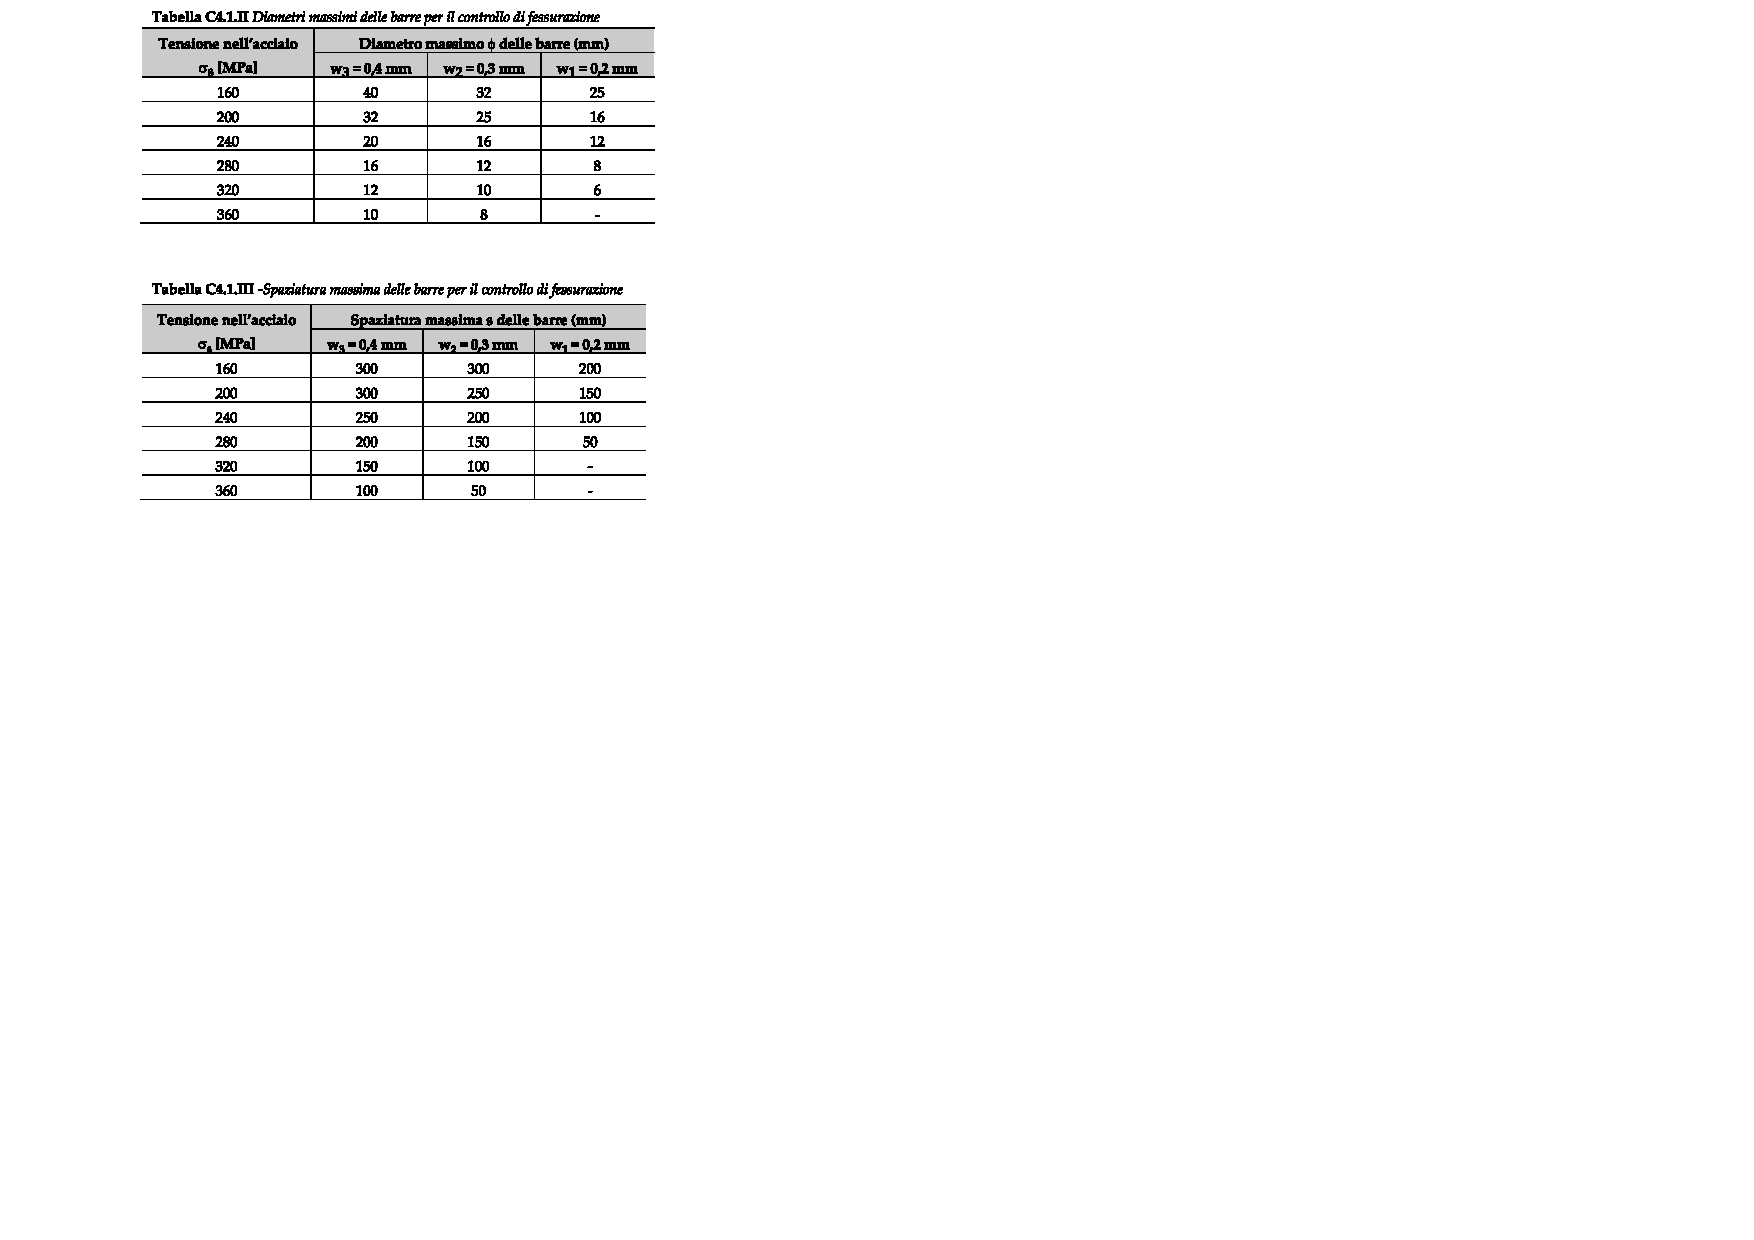
\includegraphics[width=.6\textwidth]{Tab_fessurazione_circolare}
	\caption{Tabelle estrapolate dalla \circolare}
	\label{fig:tabelleFessurazioneCircolare}
\end{figure}

Il metodo semplificato consiste nella verifica - senza calcolo diretto dell'ampiezza di fessura - andando a confrontare le tensioni $\sigma_s$ delle armature nelle compinazioni frequente e quasi pemanente con le tabelle \textbf{C4.1.II} e \textbf{C4.1.III} della \circolare (vedi figura~\ref{fig:tabelleFessurazioneCircolare}). 

La tensioni nelle armature per la sezione fessurata sono quelle calcolate nella \eqref{eq:sigmas_freq} e nella \eqref{eq:sigmas_qp}, mentre la spaziatura nella sezione in esame è $s = 57.33\,mm$.

Entrando in tabella con i valori delle tensioni nelle armature deduce che il diametro massimo delle barre tese deve essere compreso tra $32\,mm$ e $40\,mm$ per la combinazione frequente e tra $25\,mm$ e $32\,mm$ per la combinazione quasi permanente. Avendo utilizzato delle barre di armature $\Phi\,18\,mm$ il controllo sui diametri è verificato secondo la normativa italiana. La spaziatura tra le barre deve essere inferiore a $300\,mm$ e circa $250\,mm$ per le combinazioni frequente e quasi permanente rispettivamente; anche in questo caso la verifica ha esito positivo, confermando perciò quanto fatto con il metodo diretto.

\section{Stato limite di deformazione}\label{sec:trave_deformazione_sle}
Per salvaguardare l'aspetto e la funzionalità dell'opera, la normativa richiede una verifica sulla freccia a lungo termine di travi e solai calcolate in  \textit{combinazione quasi permanente} delle azioni. Il limite fissato dalle \ntc è di $\frac{l}{250}$, dove $l$ è la luce dell'elemento strutturale. Nel caso in cui fossero presenti pareti divisorie, per garantirne l'integrità il limite è ridotto a $\frac{l}{500}$.

Come per lo stato limite di fessurazione, la verifica allo stato limite di fessurazione può essere eseguite con un metodo diretto - tramite integrazione delle curvature - oppure con un metodo semplificato che limita la snellezza dell'elemento.

La campata su cui ricade la scelta è la medesima della verifica precendente (campata $C5$); l'andamento del momento flettente è quello di figura~\ref{fig:C5_momento_qp}

\begin{figure}
    \centering
	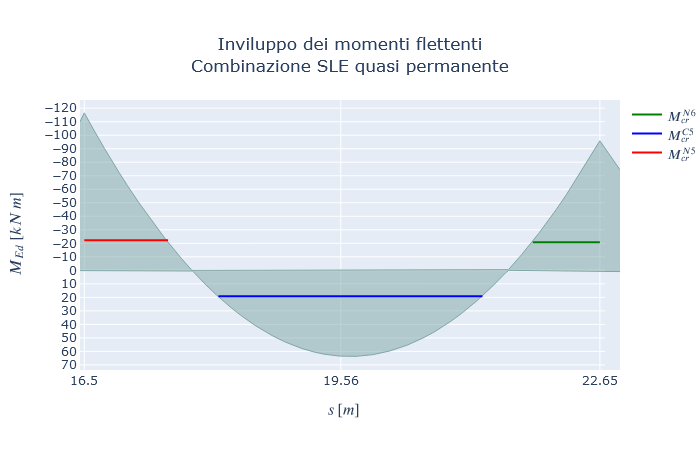
\includegraphics[height=.6\textwidth]{C5_bendingMoment_QP}
	\caption{Inviluppo dei momenti flettenti in combinazione quasi permanente - campata $C5$}
	\label{fig:C5_momento_qp}
\end{figure}

Le caratteristiche della sezione sono:
\begin{itemize}
	\item $N5$: $A_s = 6\,\Phi\,18$, $A'_s = 2\,\Phi\,18$;
	\item $C5$: $A_s = 4\,\Phi\,18$, $A'_s = 2\,\Phi\,18$;
	\item $N6$: $A_s = 5\,\Phi\,18$, $A'_s = 2\,\Phi\,18$;
\end{itemize}

Il momento di fessurazione per la verifica a deformazione vale
\begin{equation}
    \label{eq:Mcr_deformazione}
	M_{cr} = \dfrac{f_{ctm}}{h-x}\,I_{nn}
\end{equation}
dove $x$ e $I_{nn}$ sono riferiti alla sezione \textbf{non fessurata}.
\begin{align*}
    N5&:
	\begin{cases}
	    x = 267.76\,mm\\
		I_{nn} = 2.0355\cdot 10^9\,mm^4\\
		M_{cr}^{N5} = 22.32\,kN\,m
	\end{cases}\\
	C5&:
	\begin{cases}
		x = 259.27\,mm\\
		I_{nn} = 1.7667\cdot 10^9\,mm^4\\
		M_{cr}^{C5} = 19.12\,kN\,m
	\end{cases}\\
	N6&:
	\begin{cases}
		x = 263.61\,mm\\
		I_{nn} = 1.9060\cdot 10^9\,mm^4\\
		M_{cr}^{N6} = 20.72\,kN\,m
	\end{cases}
\end{align*}

Dalla figura~\ref{fig:C5_momento_qp} si può capire che il tratto compreso in $s\in[16.50, 17.50]\,m$ è fessurato ($M_{Ed}^{N5} > M_{cr}^{N5}$) mentre non lo è tra $s\in[17.50, 17.80]\,m$ essendo $M_{Ed}^{N5} < M_{cr}^{N5}$. In generale si può dividere la campata in zone. Fissando una coordinata $\xi$ che ha origine in $N5$ e corre lungo tutta la campata:
\begin{itemize}
	\item $N5F:~s\in[16.50, 17.50]\,m,~\xi\in[0, 1000]\,mm,~M_{Ed}^{N5} > M_{cr}^{N5}$, \emph{Fessurata}; 
	\item $N5N:~s\in[17.50, 17.80]\,m,~\xi\in[0, 300]\,mm,~M_{Ed}^{N5} < M_{cr}^{N5}$, \emph{Non fessurata}; 
	\item $C5N1:~s\in[17.80, 18.10]\,m,~\xi\in[0, 300]\,mm,~M_{Ed}^{C5} < M_{cr}^{C5}$, \emph{Non fessurata}; 
	\item $C5F:~s\in[18.10, 21.25]\,m,~\xi\in[0, 3150]\,mm,~M_{Ed}^{C5} > M_{cr}^{C5}$, \emph{Fessurata};
	\item $C5N2:~s\in[21.25, 21.55]\,m,~\xi\in[0, 300]\,mm,~M_{Ed}^{C5} < M_{cr}^{C5}$, \emph{Non fessurata}; 
	\item $N6N:~s\in[21.55, 21.85]\,m,~\xi\in[0, 300]\,mm,~M_{Ed}^{N6} < M_{cr}^{N6}$, \emph{Non fessurata};
	\item $N6F:~s\in[21.85, 22.65]\,m,~\xi\in[0, 800]\,mm,~M_{Ed}^{N6} > M_{cr}^{N6}$, \emph{Fessurata};
\end{itemize}

\subsection{Metodo diretto: integrazione delle curvature}
Come introdotto poco sopra, il metodo diretto consiste nell'intefrazione delle curvature. Il problema che si viene a creare è che la curvatura varia - oltre che con il momento flettente - anche con il momento di inerzia della sezione; quest'ultimo, inoltre, è diverso se la sezione è fessurata oppure non fessurata. I valori di $x$ e $I_{nn}$ in funzione delle zone sono:
\begin{align*}
    N5F&:
	\begin{cases}
		x^{N5F} = 185.67\,mm\\
		I_{nn}^{N5F} = 2.0456\cdot 10^9\,mm^4
	\end{cases}\\
	N5N&:
	\begin{cases}
		x^{N5N} = 267.76\,mm\\
		I_{nn}^{N5N} = 2.0355\cdot 10^9\,mm^4
	\end{cases}\\
	C5N1 = C5N2&:
	\begin{cases}
		x^{C5N1} = x^{C5N2}  = 259.27\,mm\\
		I_{nn}^{C5N1} = I_{nn}^{C5N2} = 1.7667\cdot 10^9\,mm^4
	\end{cases}\\
	C5F&:
	\begin{cases}
		x^{C5F} = 157.51\,mm\\
		I_{nn}^{C5F} = 1.5237\cdot 10^9\,mm^4
	\end{cases}\\
	N6N&:
	\begin{cases}
	x^{N6N} = 263.61\,mm\\
	I_{nn}^{N6N} =1.9060 \cdot 10^9\,mm^4
	\end{cases}\\
	N6F&:
	\begin{cases}
	x^{N6F} = 172.65\,mm\\
	I_{nn}^{N6F} = 1.8388\cdot 10^9\,mm^4
	\end{cases}\\
\end{align*}

Mentre nelle zone non fessurate la curvatura può essere calcolata dalla linea elastica
\begin{equation}
	\label{eq:lineaElastica}
	\chi (\xi) = \dfrac{1}{r(\xi)} = \dfrac{M(\xi)}{E\,I_{nn}}
\end{equation}
nelle zone fessurate questa non può più essere applicata. Al punto \textbf{C4.1.2.2.2} della \circolare e allo stesso modo al capitolo \textbf{7.4.3} del \ec viene proposta - per il calcolo della curvatura in fase fessurata - la seguente formulazione
\begin{equation}
    \label{eq:curvaturaFessurata}
	\chi = \zeta\,\chi_{II} + (1-\zeta)\chi_I
\end{equation}
dove $\chi_{II}$ è la curvatura considerando la sezione completamente fessurata (stato II), $\chi_I$ è la curvatura della sezione non fessurata (stato I) mentre $\zeta = 1-\beta\,\left(\frac{\sigma_{sr}}{\sigma_s}\right)^2$ è un coefficiente di distribuzione che tiene conto del tension stiffening ed è nullo per sezione non fessurata. Il termine $\beta$ è un coefficiente che tiene conto della durata di applicazione dei carichi e vale $1$ per carichi di breve durata, mentre vale $0.5$ per carichi di lunga durata (combinazione quasi permanente). Infine, la tensione $\sigma_s$ sulle armature deve essere calcolata sulla base della sezione fessurata, mentre $\sigma_{sr}$ è la tensione sulle armature generata dal momento $M_{cr}$. Il
coefficiente $\zeta$ può essere riscritto anche come
\[
\zeta = 1 - \beta\,\left(\dfrac{M_{cr}}{M(\xi)}\right)^2
\]

Le curvature allora valgono
\begin{align*}
	\chi^{N5F} &= \left(1-0.5\cdot\left(\dfrac{M_{cr}^{N5}}{M(\xi)}\right)^2\right)\,\dfrac{M(\xi)}{E_{cm}\,I_{nn}^{N5F}} + \left[ 1 -\left(1-0.5\cdot\left(\dfrac{M_{cr}^{N5}}{M(\xi)}\right)^2\right)\right]\,\dfrac{M(\xi)}{E_{cm}\,I_{nn}^{N5N}}\\
	\chi^{N5N} &= \dfrac{M(\xi)}{E_{cm}\,I_{nn}^{N5N}}\\
	\chi^{C5N1} &= \chi^{C5N2} = \dfrac{M(\xi)}{E_{cm}\,I_{nn}^{C5N1}} \\
	\chi^{C5F} &= \left(1-0.5\cdot\left(\dfrac{M_{cr}^{C5}}{M(\xi)}\right)^2\right)\,\dfrac{M(\xi)}{E_{cm}\,I_{nn}^{C5F}} + \left[ 1 -\left(1-0.5\cdot\left(\dfrac{M_{cr}^{C5}}{M(\xi)}\right)^2\right)\right]\,\dfrac{M(\xi)}{E_{cm}\,I_{nn}^{C5N}}\\
	\chi^{N6N} &= \dfrac{M(\xi)}{E_{cm}\,I_{nn}^{N6N}}\\
	\chi^{N6F} &= \left(1-0.5\cdot\left(\dfrac{M_{cr}^{N6}}{M(\xi)}\right)^2\right)\,\dfrac{M(\xi)}{E_{cm}\,I_{nn}^{N6F}} + \left[ 1 -\left(1-0.5\cdot\left(\dfrac{M_{cr}^{N6}}{M(\xi)}\right)^2\right)\right]\,\dfrac{M(\xi)}{E_{cm}\,I_{nn}^{N6N}}
\end{align*}

Per il calcolo dell'abbassamento si può applicare il \emph{principio dei lavori virtuali} dove il sistema delle deformazioni è quello descritto dalle curvature sopra calcolate, mentre il sistema delle forze è descritto da una trave a doppio appoggio caricata in mezzeria con una forza concentrata di valore unitario. Il momento generato dalla forza unitaria è


\begin{figure}
    \centering
	\begin{tikzpicture}
		\scaling{2};
		\point{n5}{0}{0};
		\point{n6}{4}{0};
		\point{a}{.5}{0};
		\point{b}{2}{0};
		\point{c}{2.5}{0};
		\point{d}{2}{1};
		
		\beam{1}{n5}{n6};
		\support{1}{n5};
		\support{2}{n6};
		\hinge{1}{n5};
		\hinge{1}{n6};
		
		\load{1}{b}[90][2];
		
		\dimensioning{3}{n5}{a}{-1.5}[$\xi_1$];
		\dimensioning{3}{b}{c}{-1.5}[$\xi_2$];
		
		\dimensioning{1}{n5}{b}{-2}[$\dfrac{l}{2}$];
		\dimensioning{1}{b}{n6}{-2}[$\dfrac{l}{2}$];
		
		\notation{1}{n5}{$N_5$};
		\notation{1}{n6}{$N_6$};
		\notation{4}{n5}{n6}[$C5$][.3];
		\notation{1}{d}{$1$}[above right];
	\end{tikzpicture}
	\caption{Sistema delle forze}
	\label{fig:plv_sistemaForze}
\end{figure}

\begin{align*}
M^\star_1 (\xi_1) &= \dfrac{\xi_1}{2}, \quad \xi_1 \in \left[0, \dfrac{l}{2}\right]\\
M^\star_2 (\xi_2) &= \dfrac{l}{4} - \dfrac{\xi_2}{2}, \quad \xi_2 \in \left[0, \dfrac{l}{2}\right]
\end{align*}
dove $l = 6.15\,m$.

Lo spostamento $\delta$ si calcola come

\begin{align*}
1\cdot \delta &= \int_{N5F} M_1^\star (\xi_1) \cdot \chi^{N5F}(\xi_1)\,d\xi_1 + \int_{N5N} M_1^\star (\xi_1) \cdot \chi^{N5N}(\xi_1)\,d\xi_1 +\\
&+ \int_{C5N1} M_1^\star (\xi_1) \cdot \chi^{C5N1}(\xi_1)\,d\xi_1 + \int_{C5F/_2} M_1^\star (\xi_1) \cdot \chi^{C5F}(\xi_1)\,d\xi_1 +\\
&+\int_{C5F/_2} M_2^\star (\xi_2) \cdot \chi^{C5F}(\xi_2)\,d\xi_2 + 
\int_{C5N2} M_2^\star (\xi_2) \cdot \chi^{C5N2}(\xi_2)\,d\xi_2 + \\
&+ \int_{N6N} M_2^\star (\xi_2) \cdot \chi^{N6N}(\xi_2)\,d\xi_2
\int_{N6F} M_2^\star (\xi_2) \cdot \chi^{N6F}(\xi_2)\,d\xi_2 = \\
	&= \left(-1.21 + 1.05\cdot 10^{-6} + 2.09\cdot 10^{-6}+ 2.13 + 3.19 + 3.32\cdot 10^{-6} + 3.97\cdot 10^{-6} -1.02\right)mm = \\
	&= 3.09\,mm
\end{align*}

Il limite fissato dalla normativa è di
\[
\delta_{max} = \dfrac{l}{250} = \dfrac{6150\,mm}{250} = 24.60\,mm
\]

Essendo
\[
\delta < \delta_{max} 
\]
la verifica sulla freccia è superata.

\subsection{Metodo semplificato}
Il metodo semplificato definito dalla \circolare consinste nel confrontare la snellezza $\lambda = \frac{l}{h}$ della trave con un valore limite riportato all'equazione \textbf{[C4.1.4]}. La normativa afferma che la verifica può essere omessa per travi o solai di lunghezza inferiore a $10\,m$ e che soddisfi
\begin{align*}
	\lambda = \dfrac{l}{h} \leq K\,\left[11 + \dfrac{0.015\,f_{ck}}{\rho + \rho'}\right]\,\left[\dfrac{500\,A_{s,eff}}{f_{yk}\,A_{s,calc}}\right]
\end{align*}

$K$ è un coefficiente correttivo che dipende dallo schema strutturale: la \textbf{Tabella C4.1.I} della \circolare definisce - per campate intermedie di travi - $K = 1.5$. I termini $\rho$ e $\rho'$ sono rispettivamente il rapporto geometrico di armatura tesa e compressa, mentre $A_{s,eff}$ è l'area di armatura tesa effettivamente presente nella sezione (valore commerciale) e $A_{s, calc}$ è l'area di armatura tesa derivante dalla soluzione delle equazioni di equilibrio al punto \ref{sec:c5} (pagina \pageref{sec:c5}).

Sostituendo
\begin{align*}
\lambda = \dfrac{6150}{500} = 12.3 &< 1.5\,\left[11 + \dfrac{0.015\cdot 25\,MPa}{\dfrac{324\,\pi\,mm^2}{(300\cdot 500)\,mm^2} + \dfrac{162\,\pi\,mm^2}{(300\cdot 500)\,mm^2}}\right]\,\left[\dfrac{500\cdot 324\,\pi\,mm^2}{450\,MPa\cdot 903.34\,mm^2}\right] = \\
&= 89.85\,mm
\end{align*}
che risulta soddisfatta. 
\cleardoublepage
